% \chapter{The First Chapter Title}
% \label{c:chapter1} Lorem ipsum dolor sit amet, consectetuer adipiscing elit.
% Nullam a tellus. Aliquam commodo dui non ipsum. Duis mollis nisi id turpis.
% Donec quis ipsum. Curabitur sed nibh. Morbi suscipit justo quis orci. Ut massa
% tortor, ultricies vitae, lacinia eu, facilisis eu, nisl. Nulla mattis urna sed
% metus imperdiet ornare. Praesent sodales. Etiam laoreet. Mauris quam magna,
% sagittis et, pharetra eget, congue vitae, arcu. Fusce sollicitudin justo.
% Suspendisse lectus. Sed lobortis dolor quis lectus scelerisque ornare. Integer
% purus. Phasellus vel elit at nibh sagittis lobortis. Aliquam iaculis malesuada
% eros. Mauris metus.

% Curabitur malesuada, pede aliquam ultrices eleifend, arcu augue cursus pede,
% vel gravida velit mauris nec sem. Etiam commodo metus vel velit. Nam aliquet
% tortor ut elit. Praesent sodales, lectus sit amet interdum vulputate, augue
% libero pretium ipsum, id congue tellus nisi posuere sem. Cras non tellus at
% magna porttitor hendrerit. Donec vehicula fermentum enim. Phasellus vel tortor
% in tellus varius condimentum. Nullam rhoncus. Morbi molestie laoreet turpis.
% Nulla ut erat. Morbi pharetra. Phasellus cursus rutrum nisl. In est. Nunc eu
% elit et purus bibendum interdum. Integer elit. Aliquam nec felis. \cite{salton83introduction}



% \section{First Section}
% \label{st:section1} Integer congue luctus justo. Curabitur libero dui,
% mollis nec, tempor vel, faucibus sit amet, massa. Fusce arcu elit, blandit sed,
% placerat venenatis, hendrerit ac, elit. Suspendisse potenti. Etiam non felis
% nec enim venenatis adipiscing. Nulla ante. Fusce dolor. Vivamus accumsan
% pellentesque eros. Maecenas pede nisl, ullamcorper vitae, venenatis sit amet,
% nonummy quis, enim. Ut in risus. Aenean nisi nisi, ullamcorper ut, posuere sit
% amet, posuere ut, turpis. Duis at est. Integer aliquam. Sed eget justo at sem
% hendrerit fermentum. Sed felis. Vestibulum tellus diam, interdum vel, vehicula
% sit amet, egestas et, lacus. Curabitur cursus felis vel sapien. In rhoncus nisi
% at orci. In lobortis varius nisi. Etiam ullamcorper libero sit amet felis. \cite{salton83introduction}

% Duis fermentum nonummy enim. In faucibus nunc. Quisque quis sem vitae ante
% condimentum imperdiet. Donec malesuada, eros non ornare sagittis, turpis pede
% hendrerit turpis, eu vestibulum mi neque ut justo. Nulla in enim eu enim auctor
% bibendum. Suspendisse in nunc. Ut adipiscing elit eu. (Figure\ref{f:fig1}).

% \subsection{First Subsection}
% \label{sst:subsection1} In tellus mauris, nonummy eget, vestibulum in,
% interdum at, nulla. Vestibulum eu justo. Vivamus lobortis pellentesque arcu.
% Aliquam enim risus, pulvinar quis, pulvinar tempor, pharetra vitae, dolor.
% Aliquam ac sapien. Aenean augue eros, malesuada nec, tincidunt eget, aliquet
% bibendum, odio. Maecenas eu est eu nisi pulvinar bibendum. Lorem ipsum dolor
% sit amet, consectetuer adipiscing elit. Pellentesque eleifend varius enim. Ut
% pharetra diam ac nulla. Aliquam a turpis ac mi semper porttitor. Vivamus
% sodales molestie nibh. Vivamus in sapien sit amet mauris sagittis lobortis.
% Aenean pretium. Suspendisse eu leo at quam vehicula aliquam. Nunc a ipsum. Sed
% placerat fringilla nibh. Aliquam sagittis. Integer a augue vitae libero
% elementum pretium. Proin metus (see Figure \ref{f:fig2}).

% Figure environment.
% \begin{figure}[!ht]
% \centering
% 
\includegraphics[width=\linewidth]{./section-chapter1/figures/uzh_logo_e_pos.pdf}
% \caption[Graphics description ABC]
% {Graphics description XYZ}
% \label{f:fig2}
% \end{figure}

% \subsubsection{First Subsubsection}
% \label{ssst:subsubsection1} Lorem ipsum dolor sit amet, consectetuer
% adipiscing elit. Nullam a tellus. Aliquam commodo dui non ipsum. Duis mollis
% nisi id turpis. Donec quis ipsum. Curabitur sed nibh. Morbi suscipit justo quis
% orci. Ut massa tortor, ultricies vitae, lacinia eu, facilisis eu, nisl. Nulla
% mattis urna sed metus imperdiet ornare. Praesent sodales. Etiam laoreet. Mauris
% quam magna, sagittis et, pharetra eget, congue vitae, arcu. Fusce sollicitudin
% justo. Suspendisse lectus. Sed lobortis dolor quis lectus scelerisque ornare.
% Integer purus. Phasellus vel elit at nibh sagittis lobortis. Aliquam iaculis
% malesuada eros. Mauris metus.

% In tellus mauris, nonummy eget, vestibulum in, interdum at, nulla. Vestibulum
% eu justo. Vivamus lobortis pellentesque arcu. Aliquam enim risus, pulvinar
% quis, pulvinar tempor, pharetra vitae, dolor. Aliquam ac sapien. Aenean augue
% eros, malesuada nec, tincidunt eget, aliquet bibendum, odio. Maecenas eu est eu
% nisi pulvinar bibendum. Lorem ipsum dolor sit amet, consectetuer adipiscing
% elit. Pellentesque eleifend varius enim. Ut pharetra diam ac nulla. Aliquam a
% turpis ac mi semper porttitor. Vivamus sodales molestie nibh. Vivamus in sapien
% sit amet mauris sagittis lobortis. Aenean pretium. Suspendisse eu leo at quam
% vehicula aliquam. Nunc a ipsum. Sed placerat fringilla nibh. Aliquam sagittis.
% Integer a augue vitae libero elementum pretium. Proin metus.


\section{A gentle introduction to credit risk}

    This section aims to give an overview of the topic that is at the heart of this paper: \textbf{credit risk}. 
    Rather than jumping straight into formal definitions, which might create difficulties in grasping with the content, 
    the reader will be first provided with real-life examples characterized by the presence of such risk. 
    Moving on, some formal definitions will be given along with a description of the agents that usually take upon 
    this risk and how they act to assess it and quantify it and finally take proper actions to mitigate it. 
    To conclude, the chapter ends with an introduction to credit risk modelling, 
    a topic that will be further explored later in the empirical analysis

    % \subsection[]{Introduction}
            
    % In a recently published online course on credit analysis \cite{creditanalysis}, 
    % the author provides a few real-life situations that occur daily and where it is possible to encounter credit risks. 
    % The following examples are based on those situations and might serve as a great starting point to understand the topic. 
    
    % \begin{example}
    %     Imagine yourself receiving a call from one of your friends that you have not heard for quite a while. 
    %     You can hear from his voice that he is really upset, and apparently, the reason for this is that 
    %     he has to pay a fine by the end of the day to avoid an additional charge, but he does not have the money 
    %     to pay at that moment. He tells you that the reason for this is that he had to cover fo huge expenses lately 
    %     and he still has not received his monthly salary. Given that, he then asks you, whether you would be kind enough to lend 
    %     him the money, promising to repay you as soon as he receives his pay. What would you do? Would you lend him the money? 
    % \end{example} 
        
    % \begin{example}
    %     Imagine to be in the same situation as above, but instead of simply being one of your friends, 
    %     the requestor is one of your colleagues at work? Would you do it in this case? Would it make a 
    %     difference if it was someone you knew well, for instance, the colleague you always work with? 
    % \end{example}

    % \begin{example}
    %     Imagine now the request to change, and instead of asking for a large sum, your colleague asks you to lend
    %     him money for a pizza without mentioning you when and how is going to pay you back. Would this make a difference 
    %     in your evaluation on whether to lend the money or not?
    % \end{example}
 
    % Although representing a very simplistic situation concerning what usually financial institutions have to deal with 
    % when they need to evaluate whether to grant the credit or not, the questions that need to be answered could be equivalent: 

    %     \begin{enumerate}
    %         \item Who is borrowing?
    %         \item How much are they borrowing?
    %         \item When will the debt be fully repaid?
    %         \item How much is there for me (either as an individual or an institution)?
    %     \end{enumerate}
    
    % Considering the last example, imagine instead that your colleague promises you to pay back the week after and on top of that,
    % he is willing to take you out for lunch. This time, what you get back is more than what you lent. 
    % In financial terms, this is also known as \textit{interest rate}. On the other hand, imagine he gives you his watch to keep 
    % until he pays you back to make the lending much safer for you. The watch in this case represents a \textit{collateral} 
    % (or a \textit{security}).

    % The procedure just introduced is usually called "\textbf{credit analysis}". According to \cite{creditanalysis}, 
    % the latter can be defined as: "\textit{the process through which the lender elaborates if he believes the counterparty is going to honour its obligations or not}". 
    % Ultimately, this determines whether or not the agent will enter in that contract, 
    % along with the relative risk associated with it, or more precisely, the \textbf{credit risk} \cite{creditriskprinciple}.

    % \subsubsection{Credit risk}

    % It is possible to find many definitions of \textit{credit risk} around.
    % \href{https://www.investopedia.com/}{Investopedia} provides us with the right one in this context:
 
    %     \begin{definition}[(Credit Risk)]
    %         \textit{the risk that a lender has to take into account due to the uncertainty related to the borrower either failing to repay a loan or to meet its obligations.} \cite{investopediacreditrisk}
    %     \end{definition}

    % In simple terms, this definition suggests that the lender should consider the possibility that a borrower 
    % will not be able to pay back the principal and the interest rate according to the initial contractual agreement. 
    % The party granting the credit should then quantify this probability and based on the result, 
    % charge a coupon rate (i.e. interest rate) to protect itself against this risk. 
    % The methods to derive the likelihood a counterparty won't be able to meet the contractual agreements are 
    % part of the broad area of \textbf{Credit Risk Modelling} \cite{bluhm2016introduction} 
    % which will be at the heart of the empirical analysis, and for this reason, it is introduced later in the paper. 
        
%     Ultimately, in the context of credit risk there are at least 3 additional points \cite{investopediacreditrisk} 
%     worth to mention which should also be considered as key takeaways from this introductory chapter:  
           
%         \begin{enumerate}
%             \item \textbf{Credit risk in every financial transaction}: although most of the times it might come naturally to associate this type of risk to transactions that occur exclusively between a party and a financial institution (e.g. mortgages, loans, credit cards, etc...), there are also situations where credit risk can be perceived between private parties (e.g. between companies and individuals: paying invoices, insurance coverage, etc..)  
%             \item \textbf{Risk assessment}: before granting new credit (as often it is the case in the business world), the bank undergoes an assessment of the borrower takes into consideration his credit history, the capabilities to repay, the capital available, the loan's conditions and associated collateral. Such evaluation has the final goal of providing an accurate prior estimate of the credit risk, which will eventually tell whether the client should get or not the obligations, with an increasing interest rate for those who are perceived as riskier. In the case of bonds, this assessment is done by credit-rating agencies that assign a triple-A (i.e \textit{AAA}) for low-risk investments, all the way down to \textit{C} for high-risk investments. Note that, although this process is almost exclusively conducted for bond products, the dataset used in the empirical analysis provides the same ratings for loans, perhaps as a result of internal procedures to assess credit risk.
%             \item \textbf{Credit risk vs. other risks}: so far it was assumed that the risk associated with the lending was purely driven by the borrower characteristics. However, in a typical lending transaction, usually, there are other types of risks kicking in: market risks (e.g. economic conditions, FX rates), country-specific risks (e.g. OECD country, emerging-markets country, etc..), operational risk, issuer risk, and so on... To keep things simple, and given the nature of the data for the empirical analysis, although it might represent a far too simplistic assumption, we will stick with it and only deal with a particular type of credit risk: the \textit{CCR (Counterparty Credit Risk)}       
%         \end{enumerate}
        
%     \subsubsection{CCR - Counterparty Credit Risk}

%     According to \href{https://www.bis.org/}{BIS - Bank for International Settlments}, \textit{CCR (Counterparty Credit Risk)} can be defined as:
    
%         \begin{definition}[(Counterparty Credit Risk)]
%             \textit{the measure of the \textbf{likelihood} that the counterparty to a transaction \textbf{might default} before meeting the contractual obligation.} \cite{basel_CCR}
%         \end{definition}

%         There is a subtle but fundamental difference between the two types of risk introduced above: 
%         when assessing the "credit risk" in general, the lender takes into account the chance that the 
%         borrower might not be able to fully repay the lender according to the contractual obligations, 
%         but do not exclude that the counterparty might cover for the remaining part in the future either. 
%         Hence, the bank is exposed (in terms of risk) only to the portion of the money lent that is perceived as being at risk. 
        
%         On the other hand, the lender might also consider the possibility that the counterparty defaults on this loan 
%         with the inability to bear the debt neither in the present nor in the future. 
%         In such a context, the lender not only has to evaluate the risk associated with the loan, 
%         but it also has to take into account the risk associated with the counterparty itself. 
%         In conclusion, if such an event occurs, and the pool of transactions with the counterparty has a positive economic value, 
%         the result would be an economic loss for the lender. 

%         As a last note, CCR is usually characterized by the bilateral risk of loss (i.e. either one of the parties involved in the transaction might default). 
%         Bilateral exposures usually factor in the uncertainty related to market movements, as part of the value of the transaction is driven by the underlying market value \cite{basel_CCR}.
%         Nevertheless, during the empirical analysis, we will assume unilateral exposures: 
%         the lender is the only one party to be exposed to the risk of the counterparty to default.


%     \pagebreak
%     \section{Basel Regulatory Framework}

%     \subsection{Introduction}
%     This section aims to introduce the key regulatory framework in the context of credit risk and more specifically, 
%     counterparty credit risk: the Basel Accord. With a walk-through in history, 
%     the objective is to make the reader aware of the reasons why lenders and companies have become increasingly regulated from this standpoint.
%     \newline\newline
%     % Reference
%     \textbf{Note}: that the content provided here is for the most part based on the information provided by the following two references: \cite{baselhistory_fu} and \cite{baselhistory_bis}

%     \subsection{Reasons for a more comprehensive framework to credit risk management}
    
%     The needs for a more comprehensive and better approach to risk management, 
%     particularly for counterparty credit risk, has emerged quite significantly 
%     after the financial crisis of 2007-2009. Since then, regulators have sharpened 
%     their existing frameworks and applied more stringent controls to 
%     the stability of financial institutions. On this line of reasoning, 
%     this section provides an overview of how regulatory requirements in 
%     the context of counterparty credit risk have evolved, with a focus on the 
%     key regulatory framework in this environment: \textbf{The Basel Accords} \cite{investopediabaselaccord}

%     After the well-known and aforementioned 2007-2009 financial crisis event, 
%     there has been an unprecedented revision of the global framework regulating 
%     the financial sector, culminating in what is known today as the \textbf{Basel III} regulatory framework.
%     Before reaching this result, the banking sector has experienced a 
%     relevant number of systemic crisis usually driven by various factors, 
%     including the miscalculation of risk, represented by inadequate capital levels 
%     to carry out their business. Each of this crisis brought some contributions and 
%     changes to the previous framework, adding up to the first version, 
%     which consisted of 30 pages, more than 1500 pages of guidelines 
%     relating to the supervision of daily banking activities. 

%     \subsection{Reasons for an independent Committee}
%     Why was the Basel Committee ever needed? 
%     To answer this question, it is necessary to go back to 1970s, 
%     when the Herstatt Bank collapsed and was put under liquidation due to 
%     enormous trades on the foreign exchange market that did not go as planned. 
%     The license was withdrawn in 1974, as losses have reached an amount equal to 
%     10 times the liquidity of the bank. However, there is more to the story: 
%     US counterparties engaging in multiple transactions with Hersatt Bank released 
%     "Deutschmark" in exchange of dollars.
%     These lenders did never see their money, essentially because of time differences: 
%     the US was still in morning trades when the bank was revoked its license. 
%     Although this is purely related to FX activities, and consequently involves 
%     also FX and market risk, this event highlighted the necessity to create a 
%     central forum for banking supervision concerning matters related also to 
%     other types of risks, such as "credit risk". To enhance the financial stability 
%     and quality of banking supervision, in 1974 multiple central banks gave rise to a 
%     centralized committee which later on took the name of "Basel Committee on 
%     Banking Supervision". The latter expanded quite significantly and as of now, 
%     it includes 45 central banks worldwide.

%     \subsection{Basel Frameworks}

%     The need for a regulatory framework for risk management was further strengthened 
%     during the 70s-80s period, when the surge in debt in the Latin American countries, 
%     combined with the rise of interest rates in the US and Europe, led the way to a 
%     series of critical debt restructuring efforts for many countries worldwide. 
%     The need for a clearer and comprehensive framework for the banking sector 
%     forced the Basel committee to issue guidelines on weighted approach to risk management. Such need was satisfied with the release of the Basel 1 framework in 1988 when for the first time in history, banks were required to weigh the capital they held against the credit risk they took. 
    
%     \subsubsection[]{Basel 1}
%     In 1988, the first regulatory framework, which later took the name of "Basel I", 
%     was released by the Basel Committee. The latter had the objective of setting up 
%     common international and shared regulations on capital adequacy supervision. 
%     The relevant aspects of the regulation are summarized in the following points:
    
%     \begin{itemize}
%         \item Credit institutions are required to classify assets into 5 different categories based on their underlying risk: from 0\% for most secured assets (e.g. cash) to 100\% for low-quality assets (e.g. private sector debt). These assets are also identified as \textbf{RWA}" (risk-weighted assets).
%         \item Definition of the so-called \textbf{Minimum Capital Requirement}: the minimum ratio of capital to risk-weighted assets (RWA). The threshold was initially set at \textit{8\%}, equally spread between most absorbing assets (i.e. \textbf{Tier-1 Capital}: examples are equity and retained earnings) and supplementary assets (\textbf{Tier-2 Capital}: examples are evaluated assets and subordinated debt). The latter includes assets that are more difficult to liquidate, and therefore less secure. This level was introduced to ensure that financial institutions had enough standalone capabilities to absorb potential losses resulting from defaulting clients.
%     \end{itemize}
    
%     Despite the effort, the first Basel Regulation had some shortcomings. 
%     These were mainly related to 3 factors: 
%     the duration of the service, 
%     the market risk and, most importantly, 
%     the counterparty risk. 
%     The introduction of amendments helped in assessing some of these issues
%     (such as the Market Risk Amendment). 
%     Nevertheless, the complexity introduced by some financial products 
%     (Credit default swaps, Complex derivatives, etc..) was drastically incrementing 
%     the risk taken by financial institutions. 
%     This situation required further adjustments with the regulation and 
%     shined a light on the ever-increasing importance of accurate methodologies 
%     to assess exposures to risk. 
    
%     \subsubsection[]{Basel 2}
%     The proposal for a replacement of the previous accord (i.e. Basel I) came in 1999 
%     and was finally released in 2004 with the name \textbf{Basel II}.
%     This comprised some of the previously mentioned and much-needed adjustments, 
%     which are summarized here:

%     \begin{enumerate}
%         \item \textbf{Minimum capital requirement}: it was developed and expanded and a new capital tier (i.e. \textbf{Tier-3}) was introduced to cover also for the market risk.
%         \item \textbf{Market discipline}: financial institutions are obliged to periodically disclose information on their risk exposures to enable much more informed decisions and constant monitoring.
%         \item \textbf{Supervisory review}: providing clear guidances on periodic assessments of an institution's capital adequacy and in case of capital pressure, it granted intervention powers
%     \end{enumerate}

%     Despite the efforts to bring more stability, 
%     the accord required time and effort before it was released. 
%     Most financial institutions had already started taking 
%     full advantage of the subprime mortgages - lending money to low credit profile - 
%     given their higher expected returns. 
%     Moreover, these institutions entered the financial crisis with too much leverage 
%     supported by the later favourable economic conditions, despite the regulatory 
%     environment that was set in place with Basel II. These events were part of a 
%     much broader series of dysfunctionality (e.g. poor governance, bad risk management, 
%     a combination of excessive credit growth and credit risk mispricing) 
%     that served as key lessons for the Basel Committee to bring substantial updates 
%     to the baseline framework. Eventually, the Committee agreed to design a reform 
%     package to outline new ways of handling credit and liquidity risk.

%     \subsubsection[]{Basel 3}
%     The agreement culminated with the publication in 2010 of what is today known 
%     as the \textbf{Basel III} framework. The aim was to improve on top of the 3 
%     pillars of the previous accord and extend them to also other areas. 
%     The key changes can be summarized in the following points:
    
%         \begin{enumerate}
%             \item \textbf{Capital conservation buffer}\cite{}: part of the common equity that, if ever breached, restricts payouts (e.g. dividends) to be used to meet the minimum common equity requirements.
%             \item \textbf{New leverage ratio}\cite{}: based on loss-absorbing capital and total institution's assets and takes into account also off-balance sheet exposures (regardless of RWA).
%             \item \textbf{Liquidity Coverage Ratio (LCR)}\cite{}: a minimum short-term liquidity ratio to provide banks with enough liquidity to cover for at least 30-days stress period.
%             \item \textbf{Net Stable Funding Ratio (NSFR)}\cite{}: a minimum long-term liquidity ratio to address maturity mismatches over the balance sheet.
%         \end{enumerate}

%     The Basel Committee realized that the approach of "one fits all" 
%     is hard to meet the expectations outlined in the framework. 
%     For this reason, it started a series of reform to condition the 
%     requirements on the institutions' size, complexity and systematic importance. 
%     This culminated in a series of on-going reform packages that are still happening 
%     today and should be published under the name of \textbf{Basel IV}.
%     \newline

%     % CONCLUSION -> FROM REGULATION -> TO HIRING IN CREDIT RISK -> RISK MODELLING -> CLOSE THE GAP WITH INFORMATION -> ASYMMETRIC IMPERFECTIONS
    
%     \pagebreak
%     \section{Credit Risk - Empirical Analysis}

%     The objective of this section is to give a high-level overview of the methodologies 
%     that the financial industry usually adopt to forecast credit losses and later leverage 
%     the data available to develop a machine-learning approach and estimate the probability 
%     that a counterparty will default on its obligation.

%     \subsection[]{Credit risk modeling}
    
%         \subsubsection{Introduction}
%         The motivations for a financial institution to develop credit risk models are much due to 
%         regulatory requirements. However, as highlighted in \cite{bluhm2016introduction}, 
%         other reasons explain the importance of internal credit risk modelling. 
%         To better understand this, let us provide a simplified, but not too unrealistic 
%         example based on the example provided in \cite{bluhm2016introduction}: 
   
%     \begin{example}

%         Imagine a bank is asked from a major tech company to provide a very huge loan in the size of \$5B. 
%         As already discussed, a credit analyst, (who for ease the example we will call Ben) will have to 
%         go through the request and see whether it is the case to grant or not this loan based on the 
%         information that he can gather. Let us assume that Ben already knows that the CEO of this company 
%         has a great friendly relationship with the CFO of the bank, and, from recent studies, 
%         he discovers that the specific sector of the company has recently experienced
%         a steady drop in sales and the bank-internal rating system suggests this company 
%         is on its way down to a sub-investment grade (i.e. classified as a risky investment). 
%         What should Ben do in this situation? Usually, the analyst has 2 options at this stage:

%         \begin{enumerate}
%                     \item \textit{Reject} the deal based on the information he gathered on the company and the relative market
%                     \item \textit{Accept} the deal BUT, protect the bank against potential losses thanks to \textbf{credit risk management instruments} (such as credit derivatives) and transfer the risk to a third-party in exchange of a fee. \cite{investopediacreditderivative}
%         \end{enumerate}

%     \end{example}

%     Hence, financial institutions have also a way out: as individuals would do through health insurance, 
%     banks can protect themselves from the underlying exposures to risk when lending to particularly risky clients. 
%     In particular, banks had already designed ways to get loan insurance in the past and usually comprises 
%     the whole bank's credit risk portfolio, and not only some critical positions. 
%     This brings directly to what in \cite{bluhm2016introduction} is perceived as the building block of 
%     credit risk modelling within a financial institution: the \textbf{expected loss}.

%     \subsubsection{Expected Loss}
%     For banks to protect against this risk, they would like to know the \textit{cost} 
%     that arises from a particular client (a group of clients when dealing with a portfolio of loans) 
%     before granting the loan, so that they can charge a \textit{premium} on the interest rate accordingly 
%     and add up to a reserve (also called \textit{expected loss reserve}) to cover for potential losses 
%     due to defaulting loans.
%     In this context, the bank is interested to know, \textit{on average}, 
%     the potential loss that might occur when lending money to a client.
%     This value is called \textbf{Expected Loss} and it is characterized 
%     by the 3 pillars of credit risk modelling \cite{bankofenglandcreditrisk}:

%         \begin{enumerate}
%             \item \textbf{Probability of Default (PD)}: the \textit{likelihood} of a default in a defined time-horizon associated to a client. Note however that this is a general definition that may vary depending on the method used to estimate such probability. For instance, under the Basel II IRB framework, the PD per rating rate is defined as the average percentage of obligators that will default over one year (i.e. the time-horizon specified in the regulation for each asset class).
%             \item \textbf{Exposure At Default (EAD)}: \textit{estimated outstanding amount} given that a client defaulted
%             \item \textbf{Loss Given Default (LGD)}: \textit{proportion of EAD} that is expected not to be recovered in case of default.
%         \end{enumerate}

%     To be mathematically rigorous, the model describing the expected loss is defined on top of a probability space ($\Omega,\Phi,\mathcal{P}$), where $\Omega$ consists of the \textit{sample space} defining all the possible events, 
%     $\Phi$ is the \textit{$\sigma$-Algebra} containing all the measurable events of the sample space (such as the information on whether an obligator default or not) and lastly, 
%     $\mathcal{P}$, the probability space, which attaches a probability to each measurable event.

%     If we declare $\textbf{\textit{D}}_{i}$ as the event that the client '\textit{i}' defaults within a time-horizon and $\mathcal{P}(D_{i})$ as the probability associated to this event, then 
%     the loss related to the obligator can be then defined as:
    
%     \begin{equation}
%         L_{i}=I*EAD_{i}*LGD_{i} \quad\mathrm{with}\quad  I = \mathrm{\textbf{1}}_{D_{i}}, \quad\mathcal{P}(D_{i}) = PD_{i}
%     \end{equation}
%     where $I$ is equal to the \textit{indicator function} of the underlying event \textit{D}. The variable takes value 1 when the 
%     event occur (i.e. default) and 0 when it does not occur. Note that this is a Bernoulli R.V., and as such, the expectation is equal to the probability of the event to occur. In other words, it is equal to the \textit{Probability of Default (PD)}. 
%     Before laying down the formula of \textit{Expected Loss}, is necessary to list down some assumptions (\cite{bankofenglandcreditrisk}, \cite{bluhm2016introduction}):
    
%     \begin{enumerate}
%         \item To keep things simple, we will assume that the 3 constituents of the loss formula (i.e. PD, EAD, LGD) are independent among each other. Despite being a more than questionable statement and far from being true in general, this setting will allow us to state the most simple formula for the \textit{Expected loss}.
%         \item To be able to simply define the expected loss over the whole portfolio of obligations, we also assume the joint distribution to be composed of independent and identically distributed R.V., each describing the expected loss of a specific obligator (\textit{i}).
%     \end{enumerate}

%     The formula of the expected loss of an obligator now comes very naturally as it is simply the expectation of the loss function defined above:

%         \begin{equation}
%             E[L_{i}]=\mathcal{P}(D_{i})*EAD_{i}*LGD_{i}
%         \end{equation}
    
%     where $\mathcal{P}(D_{i})$ represents the expectation of $I$.

%     At this point, it is possible to identify the expected loss of a portfolio as the proportion of obligators that might default over a time-horizon,
%     multiplied by the expected portion of the total expected exposures that is assumed not to be recovered if the default event occurs. More formally:

%         \begin{equation}
%             E[L_{P}]=\sum_{i=1}^{N} \mathcal{P}(D_{i})*EAD_{i}*LGD_{i}
%         \end{equation}

%     \subsubsection{Unexpected Loss}
%     Note that the formula to calculate the expected losses aims at measuring the \textbf{expected} 
%     proportion of losses due to defaulting obligators based on historical default experiences, 
%     but it does not consider the \textbf{unexpected} losses that might come up as a deviation 
%     from the average experienced losses of the past. \cite{bluhm2016introduction}. 
%     The capital held to sustain losses should then consider both, and for the sake of completeness of this chapter, 
%     the formula will be provided here:

%     \begin{equation}
%         UL_{P}=\sum_{i=1}^{N} \sigma_{i}*\varphi_{i}
%     \end{equation}
%     where $\sigma_{i}$ is the individual standard deviation of credit losses for the obligator \textit{i}, while $\varphi_{i}$ indicates the correlation between the credit losses of individual \textit{i} and all the other obligators in the portfolio.

%     After this brief parenthesis, let us go back to one of the key constituents of expected loss, the
%     \textbf{probability of default}.

%     \subsubsection{Probability of Default}

%     Predicting the probability of default is in itself a very challenging task as often it involves very complicated models that need to assign a 
%     likelihood of defaulting to each of the clients in the portfolio. To handle this task,  financial institutions have set up a division 
%     in charge of estimating the 3 main constituents of the expected loss as a way to keep the situation monitored and intervene when needed. 

%     In principle, there are many methods to estimate the probability of default, 
%     but we will list only 3 different approaches \cite{bluhm2016introduction} and, 
%     for the scope of our analysis, the focus will be posed on just one of them:
    
%             \begin{enumerate}
%                 \item \textit{Calibration from the \textbf{market data}}: calibrating default probabilities on market data is not an easy task, and for this reason, there are already ad-hoc models (such as the KVM-model) that take care of this. Another option is based on credit spreads of the product bearing credit risk.
%                 \item \textit{Calibration from the \textbf{ratings}}: default probabilities are linked with ratings (e.g. AAA,AA,\dots, BBB, \dots) which can be provided either by internal-based methodologies or by external rating agencies (e.g. Moody's, S\&P, Fitch, \dots)
%                 \item \textit{\textbf{Model-based} calibration}: as a further solution, the one used in the analysis to follow, it is possible to build a model to predict the default probabilities based on the available information on the obligation and the relative obligator.
%             \end{enumerate}
    
%     Note that, the approach taken in the analysis will be purely based on setting up a 
%     machine learning model trained on simple characteristics concerning the loans and the counterparties.
    
%     \pagebreak
%     \subsection[]{Empirical work}

%     \subsubsection*{Introduction}
%     This section presents a credit risk analysis and modelling on a portfolio of loans applying machine learning techniques. 
%     The core objective is to inspect whether given a set of characteristics on the loans and the counterparties, 
%     it is possible to accurately assess the probability of default of an obligator with the ultimate objective of decreasing 
%     the default rate of the portfolio as a whole with mutual short and long-term benefits for both the lender and the client.
    
%     \subsubsection*{Frame the problem}
%     This article \cite{frametheproblem} outlines something of paramount importance in a data science context: having a 
%     clear idea of the problem at hand is fundamental, especially when dealing with empirical data. The aim here is first 
%     defining the requests from a business perspective and then translate them to reflect on how to optimally approach these 
%     questions from a data science point of view. Following this procedure, it is possible to use statistical techniques to 
%     explore the data and provide justifiable answers.
    
%     From a managerial point of view, as a financial institution, we want to focus on assessing the default probability of 
%     single loans and, from a data science perspective, this translates into a binary classification problem. 
%     The output of the model can take two possible values:
    
%     \begin{itemize}
%         \item \textbf{1}: the counterparty is predicted to \textbf{default} 
%         \item \textbf{0}: the counterparty is predicted to \textbf{NOT default} 
%     \end{itemize} 

%     To inspect how the model performed and punish it for mistakes, it is necessary to define an error metric to minimize. 
%     Choosing an error metric much depends on the business case as well as on the data at hand, but for a classification problem 
%     the set of possible options boils down to just 3: accuracy, precision and recall. Our choice will be taken and justified later in the analysis.

%     \subsubsection*{Data collection}
%     The whole analysis is based on data \cite{kaggledataset} collected from a very popular data science online platform: Kaggle. 
%     The dataset is characterized by a panel data structure where each observation simulates credit bureau features of loans and counterparties. 
%     For convenience,  the dataset is first split into two subsets: counterparties and loans, each of which reports the respective underlying features. 
%     Finally, the dataset is combined for multivariate analysis and modelling purposes.

%     \subsection{A first glance at the data}
%     The goal of this section is to give a high-level overview of the data 
%     at hand. The dataset provides general information on 32581 loans along with
%     the characteristics of the obligators associated with each loan.
%     Let's explore them separately

%     \subsubsection*{Counterparties}
%     The counterparties are described by the following 6 features:

%         \begin{itemize}
%             \item \textit{Age}: age of the person 
%             \item \textit{Income}: personal income in \$ (dollars)
%             \item \textit{Home ownership}: whether the person owns a house or it is supplied with in any other ways (RENT, MORTGAGE, ... or other financial instruments)
%             \item \textit{Employment length}: how long (in years) the person has been employed
%             \item \textit{Person default on file}: whether in the past the person has already defaulted or not on an obligation
%             \item \textit{Credit history length}: length of the credit grant in years up until now
%         \end{itemize}

%     % cp_info FIGURE
%     From the figure [TODO] the variable "employment length" presents some missing values
%     that must be handled before proceeding into modelling.

%     % cp_head FIGURE
%     The first few observations of the dataset show some inconsistencies with the data: the first observation 
%     is characterized by a value for \textit{emplyment length} of 123 years. Let us go into more details:

%     % cp_describe FIGURE
%     A statistical summary of the numerical features allows us to further inspect the issue with the data, as well
%     as having a preliminary assessment of the distribution of each feature. In particular, some inconsistencies 
%     in the \textit{age} and \textit{employment lenght} features are spotted and consequently eliminated. 
%     A graphical representation of the univariate distribution for each counterparty's features is provided here:

%     %cp_univariate FIGURE
%     The following is a list of some of the relevant findings of the figure above:

%         \begin{enumerate}
%             \item The set of counterparties is mostly represented by people between their 20s and their 40s. The age distribution seems to have an impact on all the remaining variables.
%             \item Lower age should be the reason for having shorter employment periods and credit history length. In particular, there seems to be a great portion of unemployed people as well as a very large amount of counterparties with little-to-none credit history. Intuitively, unemployment should have a high impact on the assessment of the probability of defaults of a counterparty. 
%             \item A very small number of counterparties owns a house, while the majority is either renting or on a mortgage, or in other words, they are already sustaining some debt. Hence, the question here becomes whether these individuals have enough liquidity inflows to sustain another obligation for an extended period.
%             \item The most representative class of counterparties have not defaulted on an obligation in the past. 
%         \end{enumerate}

%     Note that the features \textit{age}, \textit{employment length} and \textit{credit history} will be discretized
%     and consequently transformed into categorical features. The observations will be then divided into multiple bins 
%     according to their underlying distribution (i.e. the categories are created based on the quantiles of the feature's distribution).
%     The objective here is to reduce the \textbf{collinearity} between the features with the hope of increasing the model's predictive powers
%     and performance.

%     \subsubsection*{Loans}
%     The loans are described by the following 6 features:

%     \begin{itemize}
%         \item \textit{Loan intent}: the reason to ask for a loan
%         \item \textit{Loan grade}: the rating associated with the loan and the relative counterparty. This variable should give us insights on the risk associated with the loan, which is usually driven by the underlying characteristics of the financial instrument (i.e. the loan) as well as the counterparty's characteristics.
%         \item \textit{Loan amount}: the amount of the loan
%         \item \textit{Loan interest rate}: the interest rate associated with the loan.
%         \item \textit{Loan status}: whether the counterparty has defaulted or not on such loan (1 is defaulted, 0 is not) 
%         \item \textit{Loan over income}:  the proportion of the loan amount concerning the income of the relative counterparty 
%     \end{itemize}

%      % loan_info FIGURE
%      An overview of the information related to these features shows some missing values for the \textit{interest rate} variable
%      and a variable called \textit{fk cp} which was introduced to reconcile counterparties with loans features 
 
%      % loan_head FIGURE
%      The first few observations of the features describing the loans do not present any relevant concern regarding 
%      data inconsistencies. Let's verify if this can be generalized to the entire dataset
     
%      % loan_describe FIGURE
%     All the numerical features seem to be within the expected range, with the expection of \textit{loan over income}:
%     this variable is calculated dividing the \textit{loan amount} with the \textit{counterparty income}. Hence, having 
%     those variables a minimum value greater than 0 simply translates into presence of inconsistencies which can be simply 
%     corrected by replacing the entire column with the original calculation.
    
%     % loan_univariate FIGURE
%     The following is a list of some of the relevant findings of the figure above:
 
%         \begin{enumerate}
%             \item The loan amount is mostly concentrated around 5-10K, which is a relatively low number if compared against the distribution of the counterparty's income.
%             \item A great proportion is classified as a "relative safe loan" (i.e. loan grade being either equal to "A", "B" or "C"). Considering this finding, along with the relatively high frequency of non-defaulting loans, it might be the case that the provided PD calibration has already a high degree of accuracy (i.e. the lender can properly distinguish between good and bad obligators). 
%             \item Despite a balanced representation of intents, "education" seems to prevail among the reasons to ask for a loan. Debt consolidation usually signals larger debt, lower interest rates, but also a great payment history with the lender. \cite{debtconsolidationinvestopedia}
%         \end{enumerate}
 
%     \subsubsection{Loan affordability}
%     Previous to granting a loan, a lender would like to know whether a counterparty will be able to sustain that loan in the 
%     future. To be able to properly assess this, a lender would require details of a counterparty's inflows and outflows 
%     as well as short-term future plans. This is usually referred to as "mortgage affordability"\cite{affordability}, as it is frequently used as one 
%     of the main determinants of a financial istitutions propensity to extend a mortage. Despite dealing with a more general type of debt
%     and not having all the information required, it is possible to define a simplified version of the \textbf{affordability} with the features 
%     provided:

%         \begin{equation}
%             affordability_{i}=\frac{(loanAmount_{i} * loanIntRate_{i})}{income_{i}}
%         \end{equation}

%     The following graph provides evidence of the importance of this variable in assessing the probability of default of a counterparty. 
%     In particular, it is possible to notice that defaulting loans presents higher affordability values, which translates into greater outflows
%     with respect to the income of a counterparty, and intuitevely, higher chances of counterpaties defaulting on such loans.
    
%     %affordability FIGURE
%     \subsection*{A combined analysis: between bivariate and multivariate analysis}

%     %TOMORROW

%     % \begin{figure}
%     %     \centering
%     %     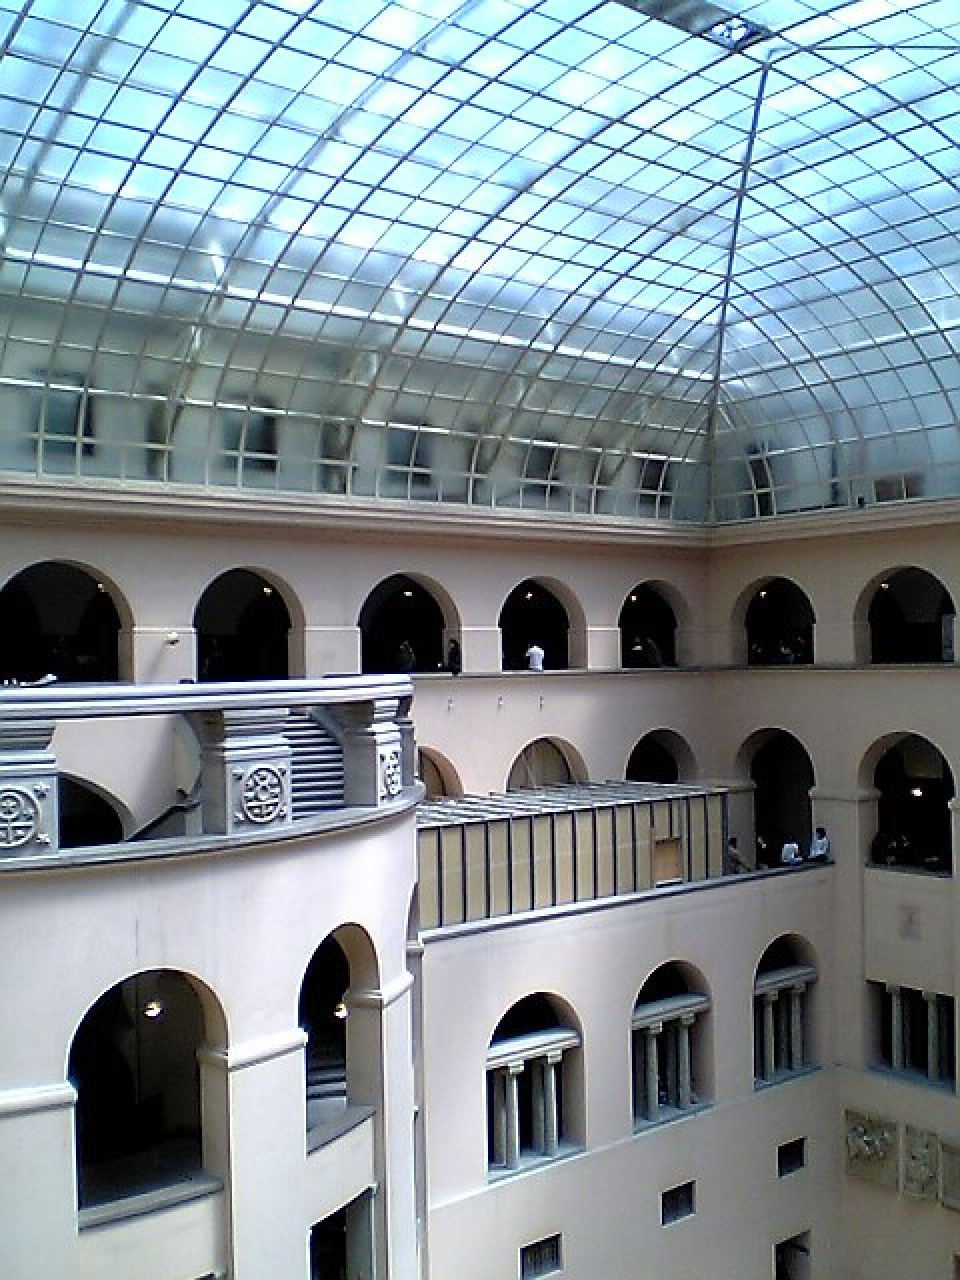
\includegraphics[height=2.0in,width=5.0in]{./section-introduction/figures/uzhlichthof.jpg}
%     %     \caption{image1 caption}
%     %     \label{f:figtag}
%     % \end{figure}
    



    

    
    








    

%     In particular, 

    

    
%     \subsubsection*{Modelling - Probability of Default}
%     After an extensive overview and analysis of the features characterizing the dataset, it is time to proceed into modelling taking into consideration the 
%     findings emerging from the previous sections. Multiple models will be implemented here: first, a logistic regression model will be fitted and optimized in order 
%      used to derive the   



%     \pagebreak
%     \section{Blockchain and asymmetric information}